\documentclass[10pt]{beamer}
\usepackage[spanish]{babel}
\usepackage[utf8]{inputenc}
\usetheme[progressbar=frametitle]{metropolis}
\usepackage{appendixnumberbeamer}

\usepackage{graphicx} % figuras
\usepackage{subfigure} % subfiguras

\usepackage{booktabs}
\usepackage[scale=2]{ccicons}

\usepackage{pgfplots}
\usepgfplotslibrary{dateplot}

\usepackage{xspace}
\newcommand{\themename}{\textbf{\textsc{metropolis}}\xspace}

\title{Inicialización de k-means - Clustering}
\subtitle{Inteligencia Computacional}
% \date{\today}
\date{}
\author{Cipolatti Edgardo, Rosales Mario, Santellán Franco}
\institute{Director: Leandro Di Persia}
% \titlegraphic{\hfill
\includegraphics[height=1.5cm]{logo.pdf}}

\begin{document}

\maketitle

\begin{frame}{Tabla de contenidos}
  \setbeamertemplate{section in toc}[sections numbered]
  \tableofcontents[hideallsubsections]
\end{frame}

\section{Introducción}

\begin{frame}[fragile]{Introducción}
\begin{itemize}

  	\item La idea es inicializar el k-Means con otros métodos m\'{a}s eficientes que elegir semillas al azar.
  \vspace{5mm}
	\item Ejecutar los métodos propuestos en diferentes bases de datos y evaluar su desempeño según diferentes medidas e índices.
\end{itemize}  
\end{frame}

\section{Métodos de inicialización de k-means}

\begin{frame}[fragile]{Métodos de inicialización de k-means}
   Los métodos de inicialización utilizados son:
   \begin{itemize}
	\item BallHall
   	\item Etiquetado
   	\item Forgy
   	\item k-means++
   	\item McQueen
   	\item McRae
   \end{itemize}
\end{frame}

\begin{frame}{Métodos de inicialización de k-means}
  \begin{itemize}
    \item \textbf{BallHall:} la primer semilla es el centro de masa de todo el dataset; posteriormente se seleccionan las restantes semillas dependiendo de una distancia d.
       	\vspace{10mm}
   	\item \textbf{Etiquetado:} se seleccionan patrones según la etiqueta $\left [  \frac{\alpha m}{k}\right ]$.
		   	\vspace{10mm}
   	\item \textbf{Forgy:} forma clusters con patrones al azar y asigna sus medias como semillas.
   	
  \end{itemize}
\end{frame}

\begin{frame}{Métodos de inicialización de k-means}
  \begin{itemize}
	\item \textbf{K-means++:} se eligen como semillas patrones en relación a una probabilidad. 
   	
   	\vspace{10mm}
   	\item \textbf{McQueen:} toma los primeros k patrones como semillas.

   	\vspace{10mm}
   	\item \textbf{McRae:} se seleccionan k semillas al azar sin repetición.
   	
  \end{itemize}
\end{frame}



\section{Medidas e Índices de evaluación de Clusters}

\begin{frame}[fragile]{Medidas e Índices de evaluación de Clusters}
   Las medidas e índices utilizados son:
   \begin{itemize}
	\item Tiempo
	\item Iteraciones
   	\item Inter-Cluster
	\item Intra-Cluster
    \item Intra/Inter
	\item Indice Davies-Boulding
	\item Indice Dunn
   \end{itemize}
\end{frame}

\begin{frame}{Medidas e Índices de evaluación de Clusters}
  \begin{itemize}
    \item \textbf{Tiempo:} Suma de tiempo requerido en crear las semillas y ejecutar k-means.
    \vspace{8mm}
    \item \textbf{Cantidad de Iteraciones:} Iteraciones realizadas por k-means.
   	\vspace{8mm}
   	\item \textbf{Inter-cluster:} Indica qué tan dispersos están los clusters.
   	\vspace{8mm}
   	\item \textbf{Intra-cluster:} Indica cuán compacto es un cluster.
   	
  \end{itemize}
\end{frame}

\begin{frame}{Medidas e Índices de evaluación de Clusters}
  \begin{itemize}
	\item \textbf{Intra/Inter:} Cociente entre los índices Intra e Inter Cluster.
   	\vspace{5mm}
   	
   	\item \textbf{Indice Davies–Bouldin:} Relación entre Intra e Inter-cluster.
   	\begin{align*}
   	\dfrac{1}{K} \sum_{i,j = 1}^{K} max \left \{ \dfrac{Intra(C_i) - Intra(C_j)}{Inter(z_i, z_j)}\right \}
   	\end{align*}
   	
   	\vspace{5mm}
   	\item \textbf{Indice Dunn:} Relación entre diámetro ($\Delta$) y distancias ($\delta$).
   	\begin{align*}
   	min_{1 \leq i, j \leq K; j \neq  i} \left \{ \dfrac{\delta (C_i, C_j)}{max_{1 \leq k \leq K} \bigtriangleup 		(C_k)} \right \}
   	\end{align*}
   	
  \end{itemize}
\end{frame}


\section{Bases de Datos}

\begin{frame}{Bases de Datos}
\centering
\textbf{Características de las bases de datos utilizadas}
\begin{table}[]
\centering
\label{DB}
\begin{tabular}{|l|c|c|c|}
\hline
\textbf{Bases de datos}                                         & \multicolumn{1}{l|}{\textbf{Dimensiones}} & \multicolumn{1}{l|}{\textbf{Clases}} & \multicolumn{1}{l|}{\textbf{Cantidad de Datos}} \\ \hline
Iris      & 4   & 3  & 150                                             \\ \hline
Nubes     & 2   & 10 & 500                                             \\ \hline
\begin{tabular}[c]{@{}l@{}}Glass \\ Identification\end{tabular} & 10  & 6  & 214                                             \\ \hline
Ionosphere  & 34   & 2  & 351                                             \\ \hline
Doughnut    & 12   & 2  & 500                                             \\ \hline
White Wine  & 11   & 7  & 500 - 4897                                             \\ \hline
\end{tabular}
\end{table}
\end{frame}


\begin{frame}{Bases de datos - Representación 2D}
\begin{figure}[htbp]
\centering
\subfigure[Iris]{\includegraphics[width=35mm]{./Imagenes/Iris.png}}
\subfigure[Nubes]{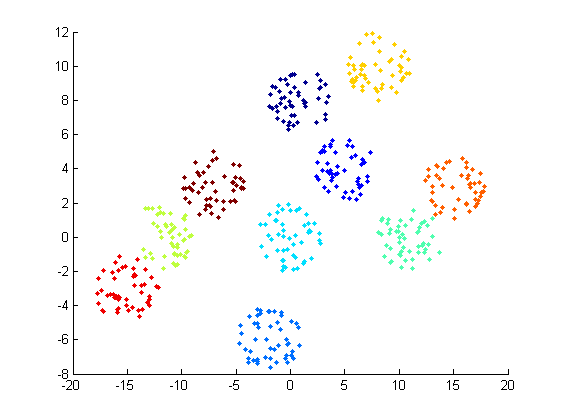
\includegraphics[width=35mm]{./Imagenes/Nube10.png}}
\subfigure[Glass]{\includegraphics[width=30mm]{./Imagenes/Glass.png}}
\subfigure[Ionosphere]{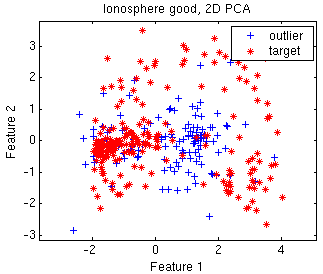
\includegraphics[width=35mm]{./Imagenes/iono.png}}
\subfigure[Doughnut]{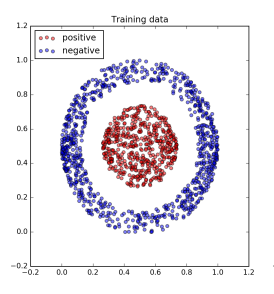
\includegraphics[width=30mm]{./Imagenes/donut.png}}
\subfigure[White Wine]{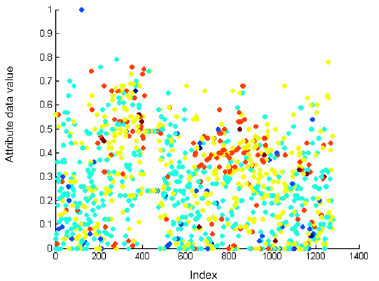
\includegraphics[width=40mm]{./Imagenes/Wine.png}}
\end{figure}
\end{frame}

\section{Resultados}

\begin{frame}{Resultados - Iris}
\begin{itemize}
\item \textbf{Iris}: $4$ atributos, $3$ clases y $150$ elementos.
\end{itemize}
\begin{figure}[htbp]
\centering
\subfigure[Iris K=2]{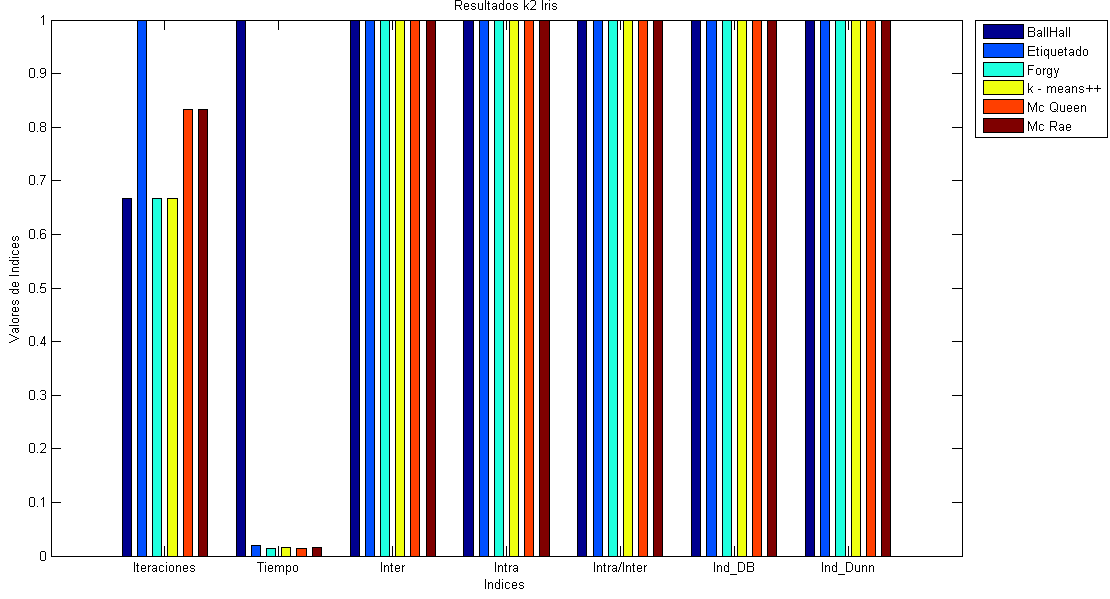
\includegraphics[width=50mm]{./Imagenes/Irisk2Global.png}}
\subfigure[Iris K=3]{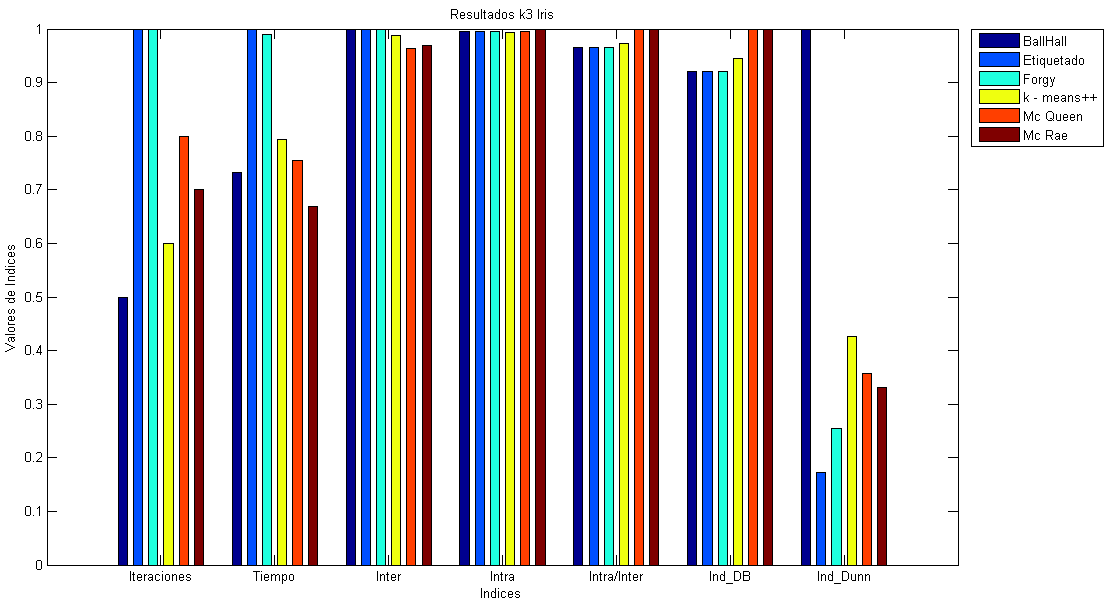
\includegraphics[width=50mm]{./Imagenes/Irisk3Global.png}}
\subfigure[Iris K=9]{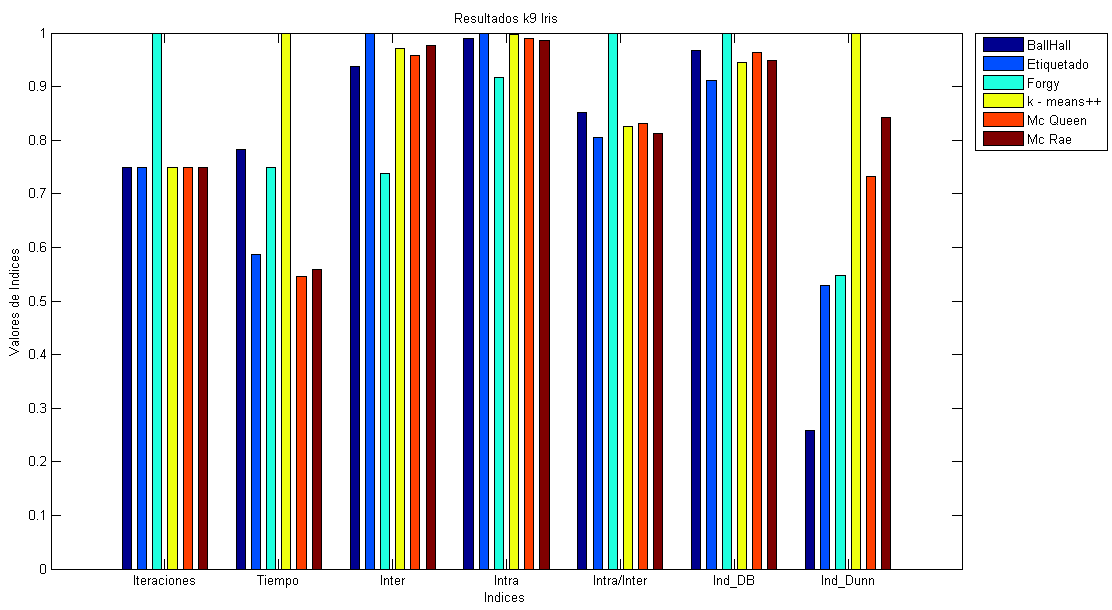
\includegraphics[width=50mm]{./Imagenes/Irisk9Global.png}}
\subfigure[Índice Dunn]{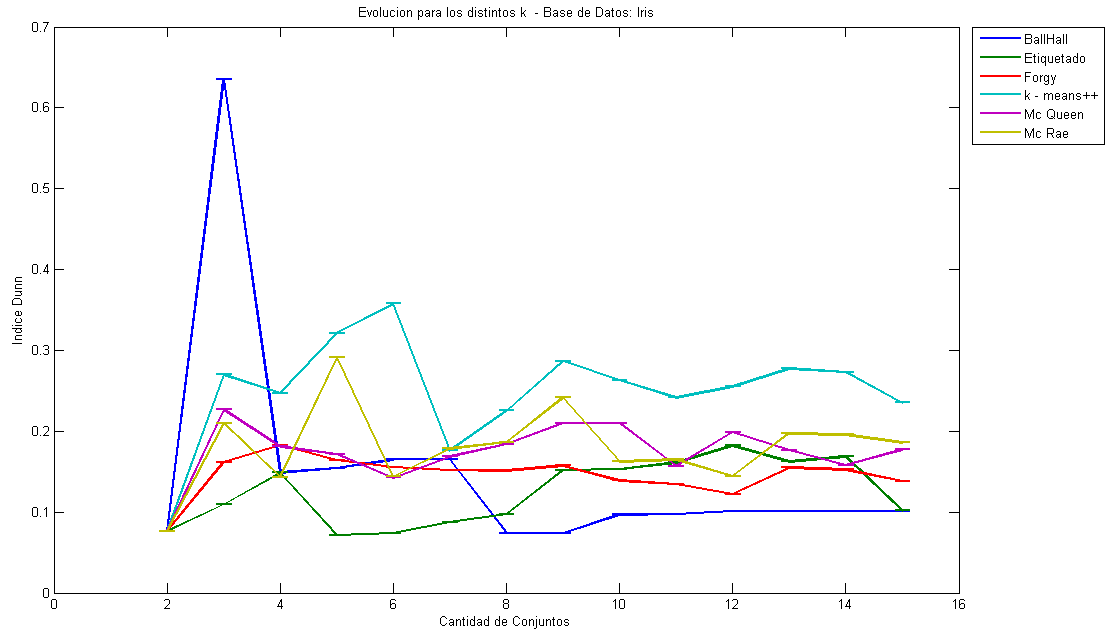
\includegraphics[width=50mm]{./Imagenes/IrisDunn.png}}
\end{figure}
\end{frame}

\begin{frame}{Resultados - Nubes}
\begin{itemize}
\item \textbf{Nubes-10}: $2$ atributos, $10$ clases y $500$ elementos.
\end{itemize}
\begin{figure}[htbp]
\centering
\subfigure[Nubes K=10]{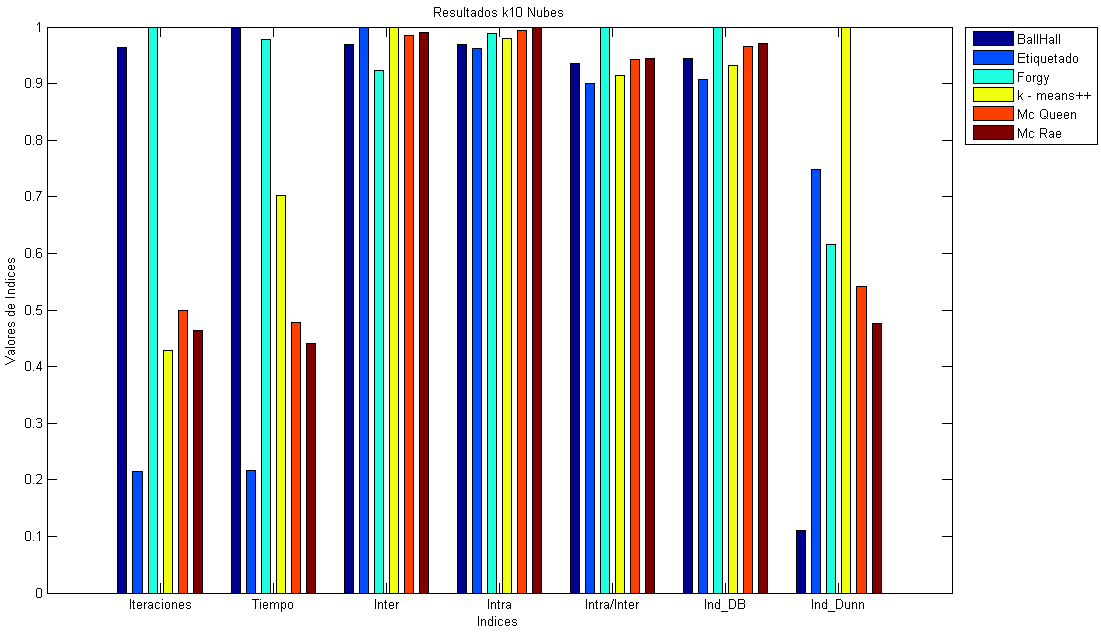
\includegraphics[width=50mm]{./Imagenes/Nubek10Global.png}}
\subfigure[Índice Intra/Inter]{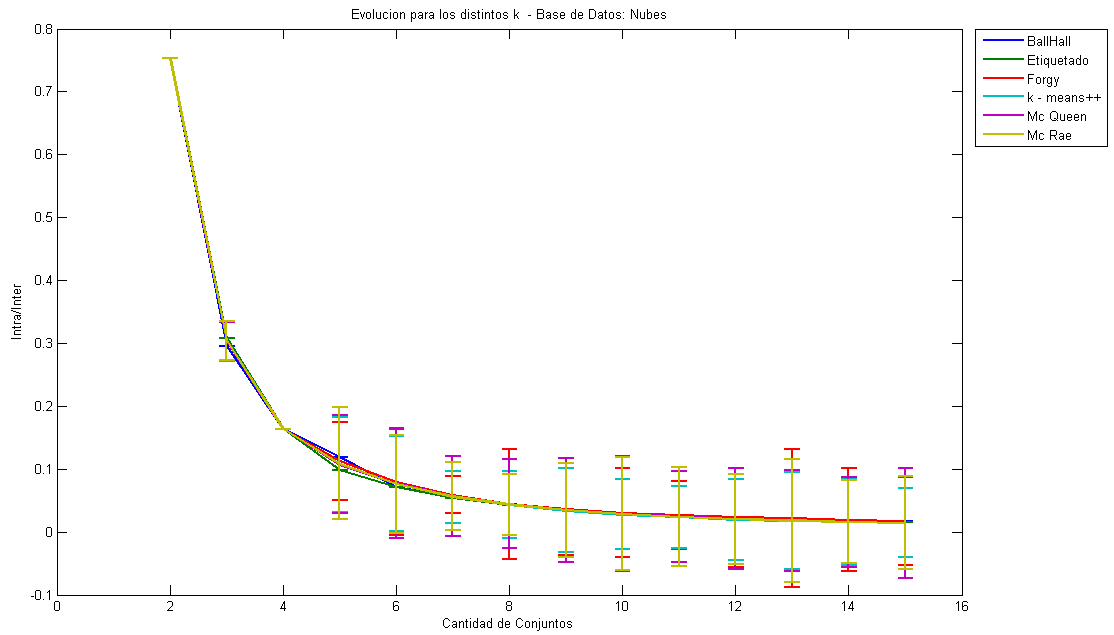
\includegraphics[width=50mm]{./Imagenes/NubesIntraInter.png}}
\end{figure}
\end{frame}

\begin{frame}{Resultados - Glass}
\begin{itemize}
\item \textbf{Glass}: $10$ atributos, $6$ clases y $214$ elementos.
\end{itemize}
\begin{figure}[htbp]
\centering
\subfigure[Glass K=6]{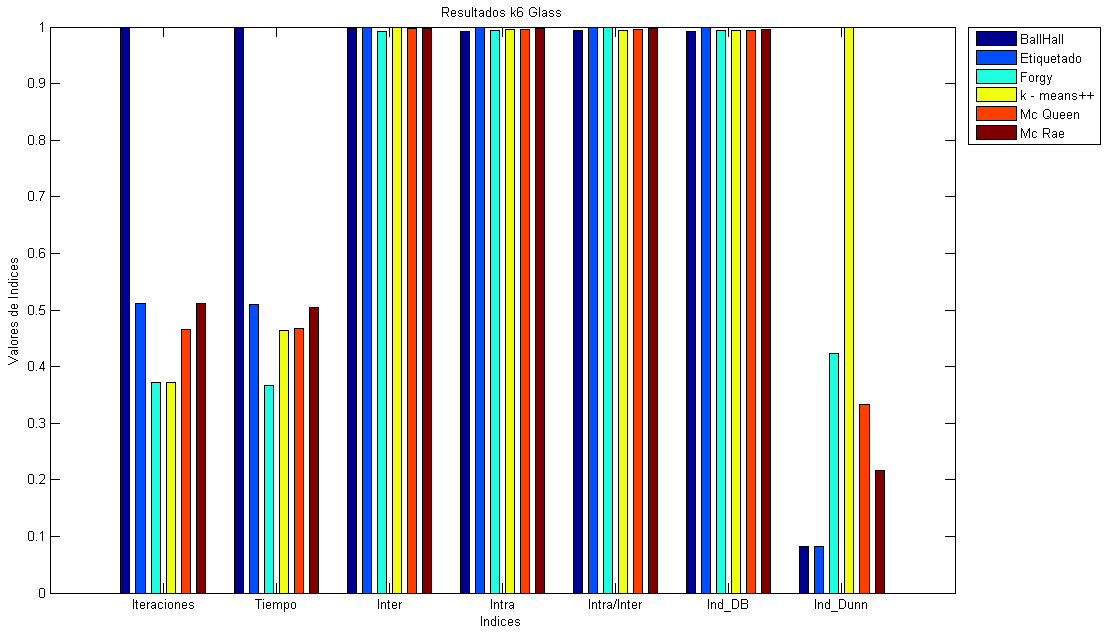
\includegraphics[width=50mm]{./Imagenes/Glassk6Global.png}}
\subfigure[Glass K=12]{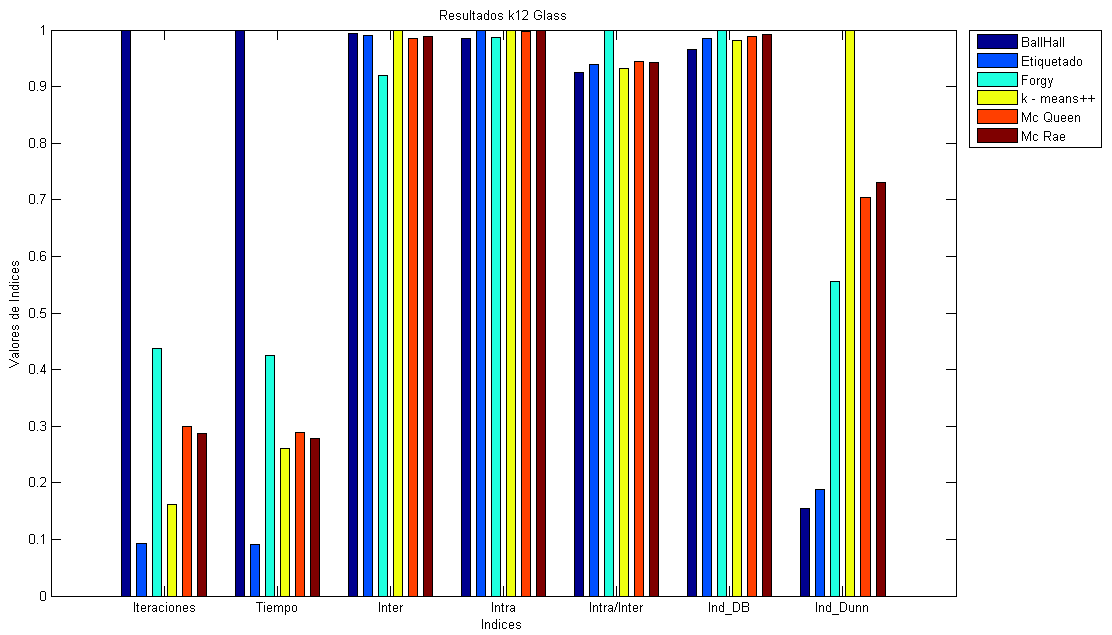
\includegraphics[width=50mm]{./Imagenes/Glassk12Global.png}}
\subfigure[Índice Dunn]{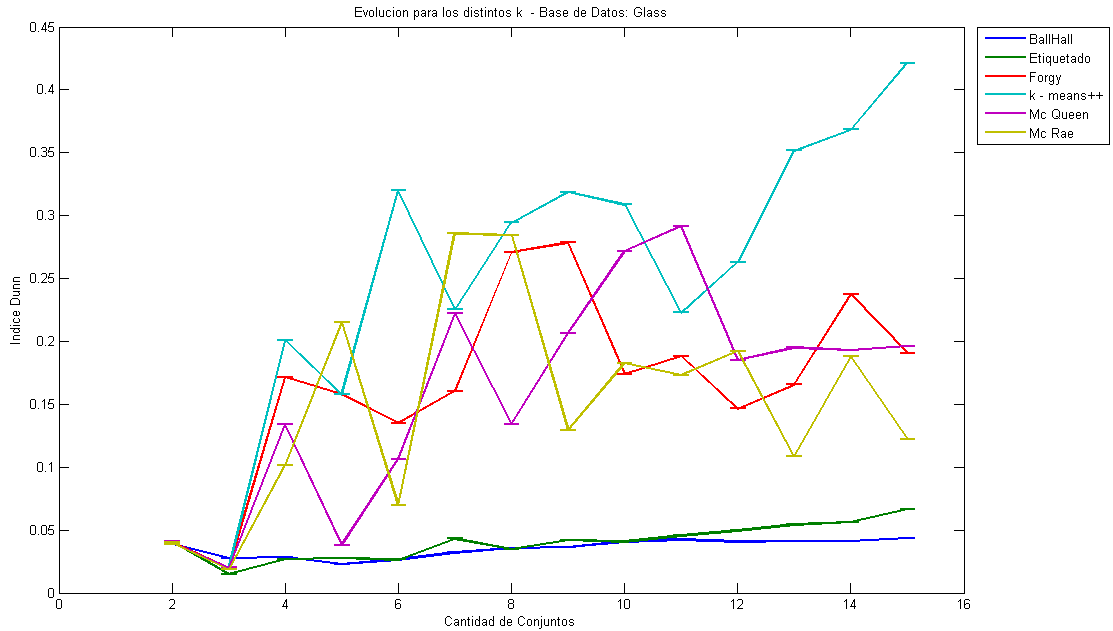
\includegraphics[width=50mm]{./Imagenes/GlassDunn.png}}
\end{figure}
\end{frame}

\begin{frame}{Resultados - Ionosphere}
\begin{itemize}
\item \textbf{Ionosphere}: $34$ atributos, $2$ clases y $351$ elementos.
\end{itemize}
\begin{figure}[htbp]
\centering
\subfigure[Ionosphere K=12]{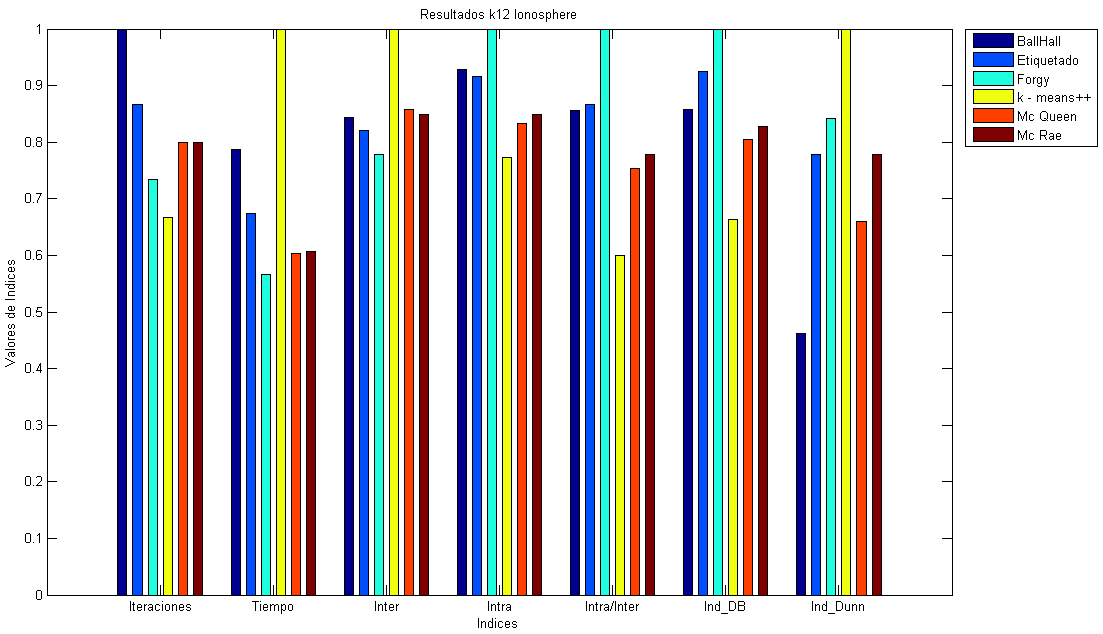
\includegraphics[width=50mm]{./Imagenes/Ionk12Global.png}}
\subfigure[Ionosphere K=14]{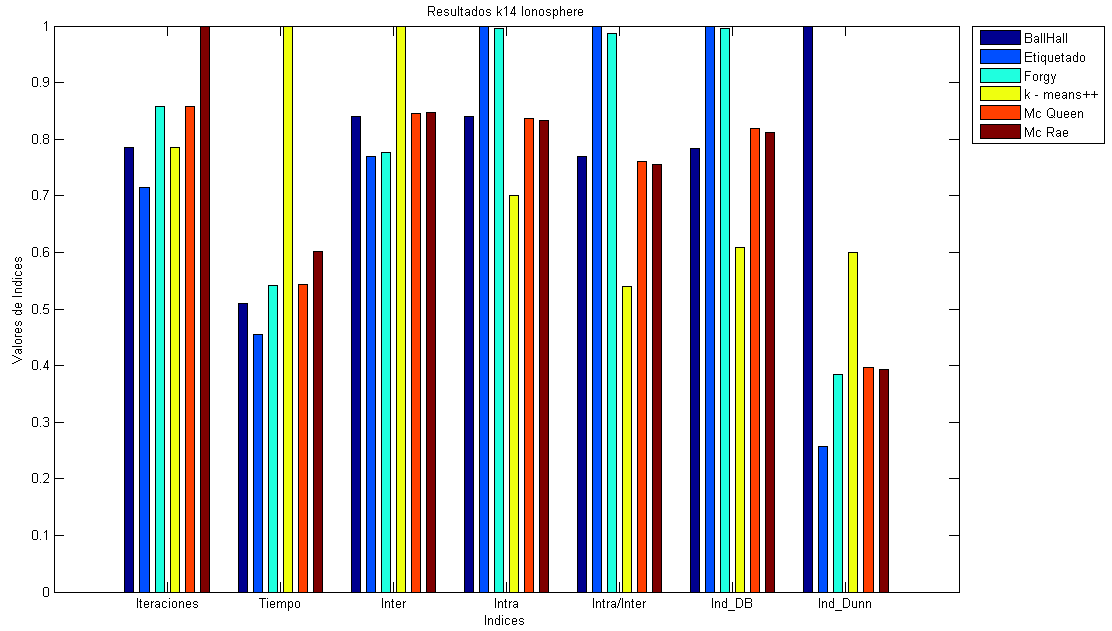
\includegraphics[width=50mm]{./Imagenes/Ionk14Global.png}}
\subfigure[Índice Dunn]{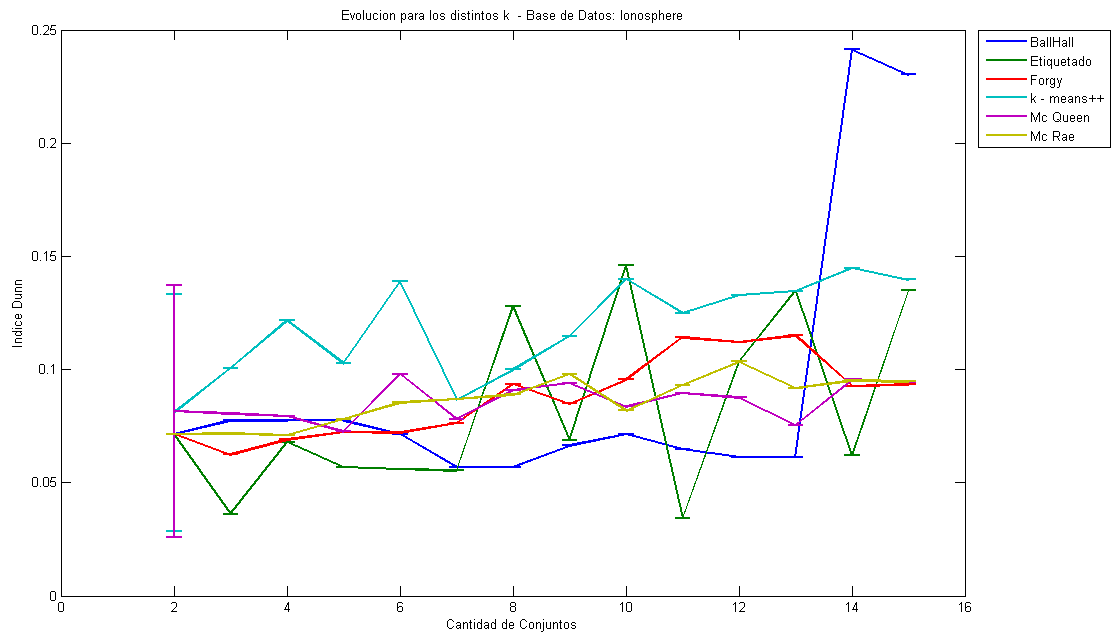
\includegraphics[width=50mm]{./Imagenes/IonDunn.png}}
\end{figure}
\end{frame}

\begin{frame}{Resultados - Doughnut}
\begin{itemize}
\item \textbf{Doughnut}: $12$ atributos, $2$ clases y $500$ elementos.
\end{itemize}
\begin{figure}[htbp]
\centering
\subfigure[Doughnut K=2]{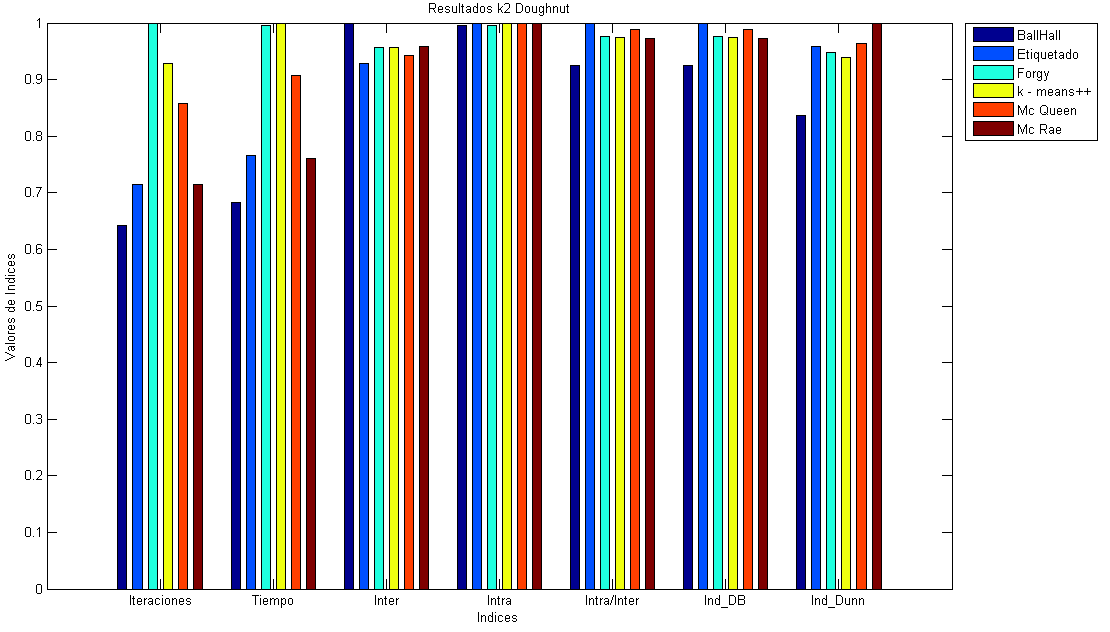
\includegraphics[width=50mm]{./Imagenes/Donak2Global.png}}
\subfigure[Doughnut K=12]{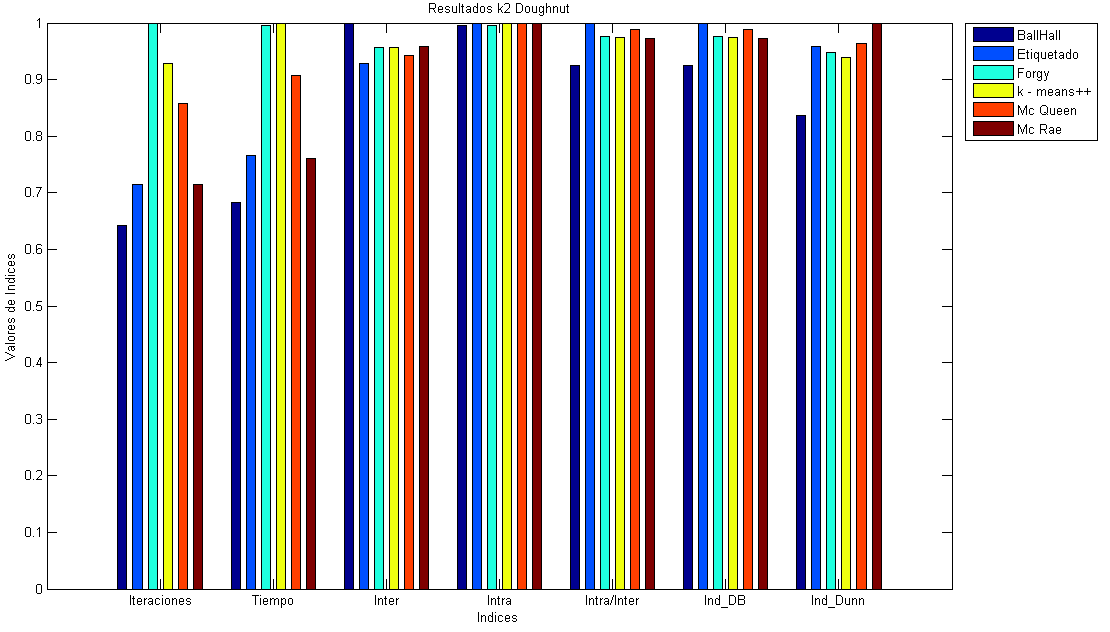
\includegraphics[width=50mm]{./Imagenes/Donak2Global.png}}
\subfigure[Doughnut K=15]{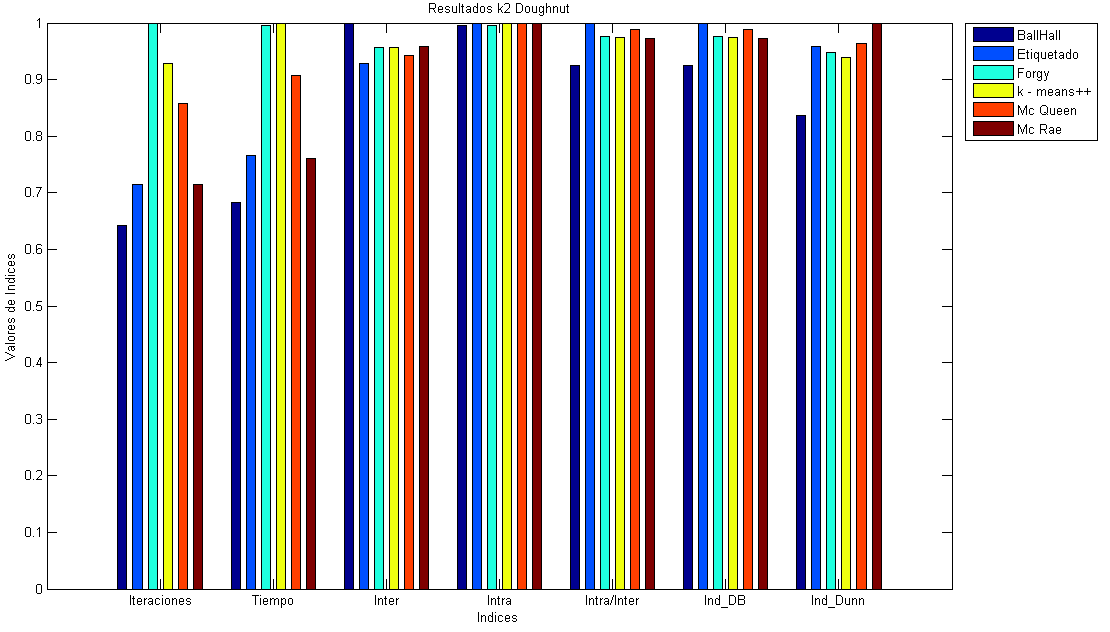
\includegraphics[width=50mm]{./Imagenes/Donak2Global.png}}
\end{figure}
\end{frame}

\begin{frame}{Resultados - White Wine}
\begin{itemize}
\item \textbf{White Wine}: $11$ atributos, $7$ clases y $500$ - $4897$ elementos.
\end{itemize}
\begin{figure}[htbp]
\centering
\subfigure[Tiempo White Wine]{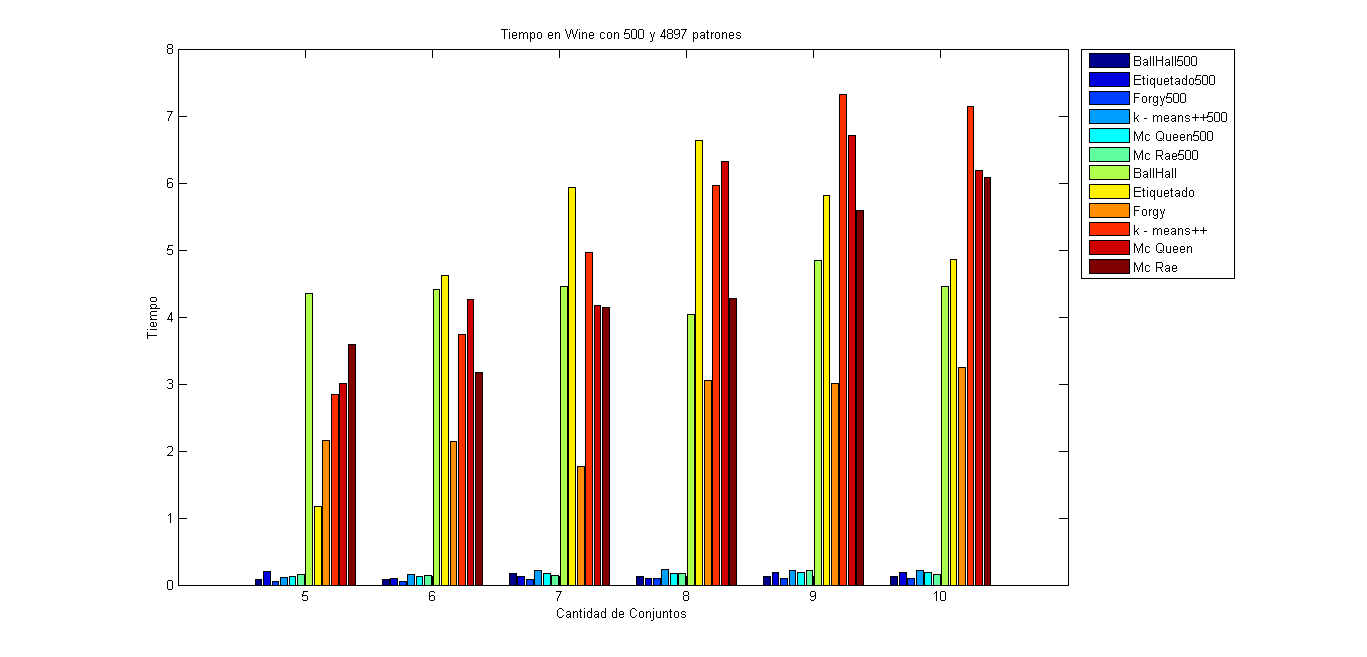
\includegraphics[width=100mm]{./Imagenes/WineTiempo.png}}
\end{figure}
\end{frame}


\begin{frame}[standout]
	¿Preguntas?
\end{frame}

\end{document}
